\documentclass[a4paper,12pt,]{article}
\usepackage[utf8]{inputenc}
\usepackage{graphicx}
\usepackage{amsmath}
\usepackage{amsfonts}
\usepackage{amssymb}
\usepackage[a4paper,top=0.1cm,bottom=1.8cm,left=1.3cm,right=1.3cm,marginparwidth=0.8cm]{geometry}
\usepackage{setspace}
\usepackage{titlesec}
\usepackage{graphicx}

\title{\large The Temperature Trends in Florida}
\author{Hongyuan Guo}
\date{October 2023}
\titlespacing*{\section}{0pt}{0.3cm}{0.2cm}

\begin{document}
\maketitle
\begin{spacing}{1.0}
\titleformat{\section}
  {\normalsize\bfseries}{\thesection}{1em}{}
\section{Introduction}
This report aims to answer the question: "Is Florida getting warmer?" by examining the correlation between the annual mean temperature in Key West, Florida, and time.
\section{Data Visualization}
The annual mean temperature trend in Key West, Florida, over the 20th century is illustrated in Fig.\ref{fig:time}.
The temperature shows fluctuations over the years, but a clear trend needs statistical verification.
\begin{figure}[htbp]
  \centering
  \begin{minipage}[b]{0.45\linewidth}
    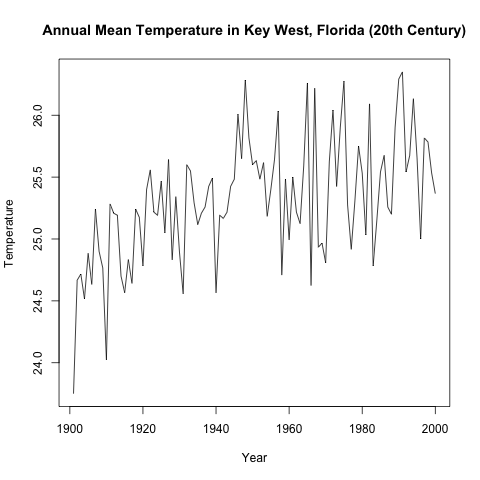
\includegraphics[width=\linewidth]{01_time.png}
    \caption{Key West Annual Mean Temperature}
    \label{fig:time}
  \end{minipage}
  \hfill
  \begin{minipage}[b]{0.45\linewidth}
    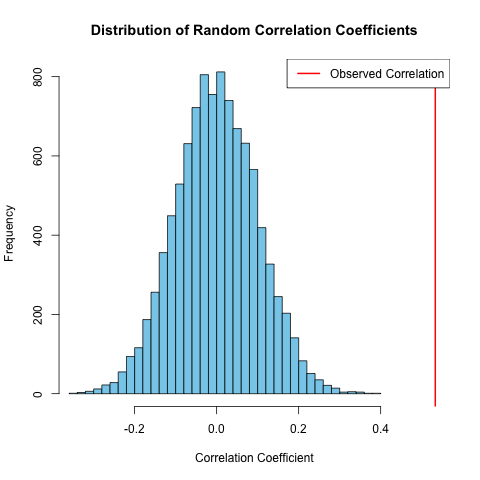
\includegraphics[width=\linewidth]{01_corr.png}
    \caption{Distribution of Correlation Coefficients from Permutations}
    \label{fig:corr}
  \end{minipage}
\end{figure}
\section{Correlation Analysis}
A permutation analysis was conducted to compute the correlation between time and temperature. Fig. \ref{fig:corr} displays the distribution of correlation coefficients derived from permutations. We define the number of iterations for the permutation as 10000, The observed correlation coefficient is highlighted in red.
\section{Results and Interpretation}
The observed correlation coefficient is significantly to the right of the distribution, implying a positive correlation. This suggests that, over time, the temperature in Florida has been increasing. 
The computed p-value of 0 further strengthens this observation, suggesting that the correlation between time and temperature is statistically significant. Thus, based on the provided data, it is reasonable to infer that Florida is indeed getting warmer over the course of the 20th century.
\section{Conclusion}
The data analysis suggests that Florida has been experiencing a warming trend throughout the 20th century. This insight underscores the importance of understanding and addressing climate change and its impacts on specific regions.

\end{spacing}
\end{document}